%------------------------------------------------------------------
%
% Vorlage für Abschlussarbeiten an der Technischen Hochschule Ingolstadt
% Bachelorarbeit/Masterarbeit
%
% Angepasst auf Seminararbeit
%
% V1 05.12.2011		Dr. Paul Spannaus
% V2 07.07.2012		Dr. Paul Spannaus
% V3 10.03.2013		Dr. Paul Spannaus
% V4 28.01.2014		Dr. Paul Spannaus
% V5 31.10.2014 		Dominik Schlecht
% 	
% -----------------------------------------------------------------
% -----------------------------------------------------------------

% Dokumentenklasse
\documentclass[a4paper,11pt,DIV=11,oneside]{scrartcl} % 

% Packages
%Datum und Uhrzeit
\usepackage{datetime}

%Encoding
\usepackage[utf8]{inputenc}
\usepackage{lmodern}

%Graphikpakete
\usepackage{graphicx}
\usepackage{xcolor}
\usepackage{tikz}
\usetikzlibrary{arrows, snakes, backgrounds}
\usepackage{wrapfig}

% Farben der THI
\definecolor{THIblue}{rgb}{0.0078,0.1176,0.4705}

\usepackage[ngerman]{babel}

%Zitierumgebung
%\usepackage{cite}% Zitieren
%\usepackage[backend=biber,]{biblatex}
%\usepackage{bibgerm}% Literatur in Deutscher DIN
\usepackage[babel,german=quotes]{csquotes}
\bibliography{ref/ref_liste} % Pfad und Datei der Ref-Datenbank

%URL-Umgebung
\usepackage{url}
\renewcommand{\UrlFont}{\small\tt\color{THIblue}}

%Mathematik
\usepackage{amsmath}
\usepackage{amssymb}
\usepackage{mathtools}

%Quellcode
\usepackage{listings}
\lstset{literate=%
    {Ö}{{\"O}}1
    {Ä}{{\"A}}1
    {Ü}{{\"U}}1
    {ß}{{\ss}}1
    {ü}{{\"u}}1
    {ä}{{\"a}}1
    {ö}{{\"o}}1
    {~}{{\textasciitilde}}1
}

\definecolor{gray}{rgb}{0.5, 0.5, 0.5}
\lstset{% general command to set parameter(s)
	basicstyle=\tiny\ttfamily,%\small, % print whole listing small
	keywordstyle=\color{THIblue}\bfseries\underbar,% underlined boldblack keywords
	identifierstyle=, % nothing happens
	commentstyle=\color{green}, % white comments
	stringstyle=\color{red}\ttfamily, % typewriter type for strings
	showstringspaces=false, % no special string spaces
	%numbers=left,
	%numberstyle=\color{gray},
	%numbersep=5pt,
	captionpos=b,
	breaklines=true}
	
% Define Language
\lstdefinelanguage{log}
{
  % list of keywords
  morekeywords={
    idVendor,
    idProduct,
    bInterfaceClass,
    bInterfaceSubClass,
    bInterfaceProtocol
  },
  sensitive=false, % keywords are not case-sensitive
  %alsodigit={0482},
  morecomment=[l]{//}, % l is for line comment
  morecomment=[s]{/*}{*/}, % s is for start and end delimiter
  morestring=[b]" % defines that strings are enclosed in double quotes
}

\lstdefinelanguage{tikz}
{
  % list of keywords
  morekeywords={
	above,
	align,
  	begin,
	below,
  	caption,
	draw,
	end,
	every,
	fill,
	label,
  	line,
	minumum,
	node,
	rectangle,
	right,
	scale,
	size,
  	style,
	of,
  	width,
  	xshift,
  	yshift
  },
  sensitive=false, % keywords are not case-sensitive
  %alsodigit={0482},
  keywordstyle=\color{THIblue}\bfseries,
  morecomment=[l]{//}, % l is for line comment
  morecomment=[s]{/*}{*/}, % s is for start and end delimiter
  morestring=[b]" % defines that strings are enclosed in double quotes
}

%Microtypographie
\usepackage{microtype}

%Kopf und Fußzeilen
\usepackage{scrpage2} 	% Kopf & Fußzeile im KOMA Stil
\pagestyle{scrheadings}	% Aktiviert Verwendung vordefinierter Kolumnentitel
\clearscrheadfoot 		% alle Standard-Werte und Formatierungen löschen
\setkomafont{pagehead}{\scshape}	% Schriftart in Kopfzeile, \scshape = Kapitelchen
\automark[chapter]{section} % [linke Seite]{rechte Seite}
%\ohead{\def\pagestyle{PDTS}{\hrulefill
\includegraphics[width = 6cm]{bilder/thi_logo_quer_cropped}}}
\ohead{
\includegraphics[width = 6cm]{bilder/thi_logo_quer_cropped}}

%\ihead{\textsc{Abschlussarbeit}}
\ihead{\headmark}

%\setheadwidth[0pt]{textwithmarginpar}
\ofoot{\vspace{-0.3cm} \pagemark} 						
\ifoot{\vspace{-0.3cm} Dominik Gunther Florian Schlecht} 
				
%\setheadtopline{.4pt}				
\setheadsepline{.2pt}
\setfootsepline{.4pt}	% Trennlinie Fußzeile und Textkörper

%------------------------------------------------------------------
%% Längenanpassungen
%------------------------------------------------------------------
\setlength{\headsep}{10mm}		% Textabstand zur Kopfzeile
\setlength{\footskip}{15mm}		% Abstand zur Fußzeile
\setlength{\parindent}{0em}		% Einzug nach Absatz

%%-------------Allgemeine Definitionen----------------------------------
% Farbige Aufwertung der berschriften
\addtokomafont{chapter}{\color{THIblue}}
\addtokomafont{section}{\color{THIblue}}
\addtokomafont{caption}{\color{THIblue}}
\addtokomafont{subsection}{\color{THIblue}}
\addtokomafont{subsubsection}{\color{THIblue}}
\setkomafont{captionlabel}{\color{THIblue}}

%Hyperref
\usepackage[
		pdftex,
		linkcolor=THIblue,			% Farbe der Verlinkung
		linktocpage=true,			% Im TOC wird Seitenzahl verlinkt(true),bzw. Text(false)
		colorlinks=true,			% 'true' keinen Kasten um Link
		citecolor=THIblue,
%		pdfhighlight=/P,
%		bookmarks,
%		hyperfigures=true,
%		citebordercolor={0 0 1},
%		linkbordercolor={0 0 1},
%		menubordercolor={0 0 1},
%		backref=true,
%		pagebackref=true,
%		bookmarksopen,
%		bookmarksnumbered,
%		pdfpagelabels=false,
%		pdfstartpage=1,
%		pdfstartview=Fit,			% Modus beim Öffnen (Fit = An Seitengröße anpassen)
		pdftitle={Umgehen von USB-Deskriptor basierten USB-Policies am Beispiel einer virtuellen Umgebung},
		pdfauthor={Dominik Schlecht},
%		pdfstartview=Fit,
%		pdfdisplaydoctitle=true,
%		plainpages=false
			]{hyperref}  

%------------------------------------------------------------------
% Wichtige Definition für Aufteilung von Formelverzeichnis und Abkürzungsverzeichnis
%------------------------------------------------------------------

% Nomenklaturverzeichnis, Formelzeichenliste Anpassungen für nomenclature: damit lassen sich zwei getrennte Symbolverzeichnisse anlegen, ziehmlich cool!
\usepackage[intoc,compatible,german]{nomencl}	
		\renewcommand{\nomgroup}[1]{	\ifthenelse{\equal{#1}{A}}{\item[{\normalfont\sffamily\bfseries\LARGE\textcolor[rgb]{0,0.112,0.47}{Abkürzungen{\phantom{\Huge $\frac{\frac{\frac{A}{a}}{a}}{\frac{a}{a}}$}}}}]}{	\ifthenelse{\equal{#1}{A}}{\item[{\normalfont\sffamily\bfseries\LARGE\textcolor[rgb]{0,0.112,0.47}{Formelzeichen{\phantom{\Huge $\frac{A}{\frac{a}{a}}$}}}}]}{}}}
		
%------------------------------------------------------------------
%% Anpassung von Abständen, Längen vom Nomenclaturverzeichnis (Abkürzungs- und Formelverzeichnis)
%------------------------------------------------------------------

% Abstand zwischen Einträgen im Symbolverzeichnis (-\parsep = 0)
\setlength{\nomitemsep}{-\parsep} 
\setlength{\nomlabelwidth}{5em}	
\renewcommand{\nomlabel}[1]{#1 \dotfill}  % Punkte im zwischen Nummer und Kapiteleintrag


%%-------------Silbentrennung--------------------------------------
\hyphenation{}

%%-------------Index-----------------------------------------------
\makeindex

%-----------------------------------------------------------------
%---------------Dokumentenbeginn----------------------------------
%-----------------------------------------------------------------
\begin{document}
	
% Titelseite
\begin{titlepage}

\phantom{tmpText}

\vspace{1cm}

\begin{figure}[h!]
\centering

\includegraphics[width=\textwidth]{bilder/thi_logo_cropped.pdf}
\end{figure}

  \begin{center}

%\vspace{1cm}
    
    
    \textbf{{\large Seminararbeit/Whitepaper} \\[3ex]
    {\LARGE Malwareanalyse} \\[1ex]
    %
    \vfill
    %
    angefertigt von} \\
    \begin{tabular}{ll}
    	Name: & Dominik Gunther Florian Schlecht\\
    	Matrikelnummer: & 00032209\\[2ex]
    	\multicolumn{2}{c}{\textbf{Betreuer:}}\\
    	Technische Hochschule Ingolstadt: & Prof. Hahndel
    \end{tabular}\\[2ex] %Vorname Nachname
    %
    \vfill
    %
    Ingolstadt, \today
  \end{center}
\end{titlepage}

	%\cleardoublepage
	\pagenumbering{roman} % Nummerierung

	% Erklärung
\section*{Erklärung}
Hiermit erkläre ich, dass ich die vorliegende Seminararbeit selbstständig und ohne fremde Hilfe verfasst habe. \\[5ex]
Die verwendeten Quellen sowie die verwendeten Hilfsmittel sind vollständig angegeben. Wörtlich übernommene Textteile, übernommene Bilder und Zeichnungen sind in jedem Einzelfall kenntlich gemacht. \\

\includegraphics[scale=.2]{bilder/unterschrift.png}\\
Ingolstadt, \today	
	
	\newpage	
	%\include{chapter/thanks_statement}
	\tableofcontents % Inhaltsverzeichnis
	\newpage
%---------------Hauptteil-----------------------------------------
	\pagenumbering{arabic} 	% Neunummerierung des Hauptteils
	\setcounter{page}{1}	% Wieder bei 1 Anfangen
	\chapter{Einleitung}
TODO
	\subsection{Physikalisches Betriebssystem}
Als Grundsystem wurde ein Linux verwendet. Dies hat den Vorteil, dass ein Großteil der sich derzeit im Umlauf befindlichen Malware für Windows konzipiert ist. (Ebenso steigt der Anteil der Malware für mobile Betriebssysteme stetig, diese werden hier jedoch nicht behandelt.) Als unkompliziertes, wandelbares und trotzdem hoch modifizierbares System wurde Debian 8 gewählt. Versuche mit z.B. Gentoo zeigten Probleme mit der verwendeten Virtualisierungslösung. 

\subsection{Virtualisierungslösung}
Es gibt viele Vorteile für die Nutzung einer Virtualisierungslösung bei der Malwareanalyse, jedoch auch Nachteile. Vorteilhaft ist vor allem das erstellen von sogenanneten Snapshots, welche einen bestimmten Zustand eines Systems aufzeichnen und es möglich machen, diesen später wieder herzustellen. Zudem wird das Host-System vor der Malware geschützt. Ein Nachteil ist, dass moderne Malware immer häufiger überprüft, ob sie in einer virtuellen Umgebung ausgeführt wird. Falls ja, werden oft andere Funktionen ausgeführt, um die ursprüngliche Funktion zu verschleiern. Insgesammt überwiegen aber die Vorteile den Nachteil. Falls die Malware auf die virtuelle Umgebung prüft, muss geprüft werden, ob über Prüffunktion über den Disassembler deaktiviert oder umgangen werden kann.

Als Virtualisierungslösung wurde VMWare Workstation 11 genutzt. Diese bietet gerade im Bereich der Netzwerkmodifikation weitere Möglichkeiten gegenüber der kostenlosen Variante Virtualbox von Oracle. Die Workstation kann von der offiziellen Webseite heruntergeladen und für 30 Tage kostenlos getestet werden.

\subsection{Virtuelles Betriebssystem}
Als virtuelles Betriebssystem wurde Windows 7 Pro verwendet. Dies ergibt sich einfach daraus, dass Windows 7 derzeit mit eines der meistverbreiteten Betriebssysteme ist und Malware meistens für Windows konzipiert ist.

Zudem wurde 32-bit als Architektur gewählt, um die Komapatibilät mit Tools wie Cukoo siche zu stellen. Außedem wurden sowohl das UAC, Updates sowie die Firewall deaktiviert, um der Malware eine Möglichst einfache Umgebung zu bieten. Die VMWare-Tools wuden absichtlich nicht installiert, da dies einer Malware eine sehr einfache Möglichkeit bieten würde, die Umgebung zu erkennen.

Diese Konfiguraton wird als Grundimage verwendet.

\subsection{Disassembler}
Als Disassembler wurde IDA PRO Free (Version 5.0) verwendet. Diese Version reicht für grundliegende Analysen, jedoch sind die möglichen Anwendungen auf 32-bit begrenzt. Da Malware jedoch so konzipiert ist, dass ein möglichst breites Spektrum an Geräten angegriffen werden kann, ist diese zumeist ebenfalls 32-bit. Um mit IDA PRO Free 64-bit Malware zu analysieren, ist eine kostenpflichtige Version notewendig. Als Alternative zu IDA PRO Free kann Hopper in Betracht gezogen werden. Hopper gibt es ebenfalls in einer kostenfreien Version, die Stärke liegt jedoch in der kostenpflichtigen Lizenz, welche ähnliche Features bietet wie IDA PRO, jedoch wesentlich billiger und somit auch für Privatpersonen erschwinglich ist. Zudem bietet Hopper den Vorteil, dass es vorgefertige Versionen für Windows, OS X und Linux gibt. IDA Pro (Free) liegt nur für Windows vor, ist jedoch über Wine relativ einfach auf Linux installierbar.

\subsection{Weitere Tools}
\subsubsection{RegShot}
\subsubsection{Resoucehacker}
\subsubsection{PEView}
\subsection{Webseitn}
\subsubsection{Virustotal}
\subsubsection{Malwr}
	\section{Infektionsweg}
In dieser Arbeit wird eine Malware, die über E-Mail verteilt wurde, analysiert. Die Mail ist im Anhang, Abbildung \ref{img:EMail}, dargestellt. Das Design ist am Speditionsunternehmen \textit{UPS} orientiert\footnote{\url{http://www.ups.com/de}}. Auch der Absender \textit{UPS express [mailto:vorname\_nachname@smtp.acenet.hu]} sowie der Titel \textit{UPS - Zustellbenachrichtigung, Kontrollnummer 635M6265282635} sind passend gewählt. Öffnet man den Link in der E-Mail wird eine Zip-Datei Namens $ups\_webtracking\_1S63A0003659818362.zip$ heruntergeladen, welche die hier analysierte Malware enthält.
	\addtocontents{toc}{\protect\setcounter{tocdepth}{2}}
	\section{Statische Analyse}
Die statische Analyse beschäftigt sich mit der Untersuchung der Malware, ohne diese auszuführen. Dies geschieht meist über Tools, welche die im Binary enthaltenen Informationen auslesen. Im folgenden werden verschiedene Methoden aufgezeigt, um die Malware statisch zu analysieren, ohne das Gastsystem einem Risiko zu unterziehen.

\subsection{Identifikation des Samples}
Zu aller erst wird das Zip-File aus der E-Mail gesichert und ein Hash erstellt, um das Sample in Zukunft auch unter einem anderen Namen identifizieren zu können. Der Hash wurde hier über die Software \textit{winMD5Free}\footnote{\url{http://winmd5.com/}} in der Version 1.20 genutzt. Alternativ hätte man unter Linux das Tool \textit{md5sum} nutzen können 
\begin{lstlisting}
ups_webtracking_1S63A0003659818362.zip
	--> 81397589ad7bf0a7faecf977644b1486
\end{lstlisting}
Die Datei wird im folgenden Text kurz \textit{8139} genannt. Um zu verifizieren, dass es sich bei der Datei \textit{8139} wirklich um ein Archiv handelt, wendet man in einem \textit{Linux}-System das \textit{File}-Kommando an. Wie in der Abbildung \ref{img:FileAufZip} zu sehen ist, bestätigt das \textit{File}-Kommando den Verdacht, dass es sich hier um ein Archiv handelt.
\begin{figure}[htbp]
	\centering
	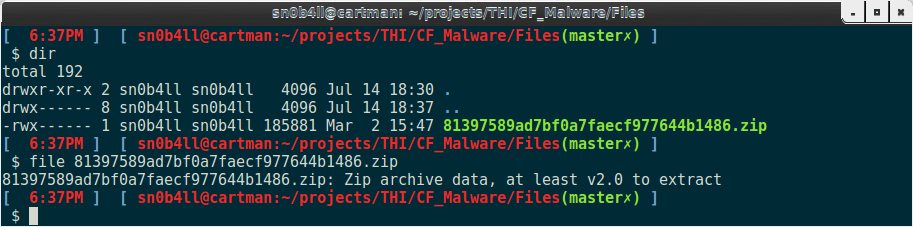
\includegraphics[width=\textwidth]{bilder/statischeAnalyse/fileAufZip.png}
	\caption{Anwendung des File-Kommandos auf die Datei \textit{8139}}
	\label{img:FileAufZip}
\end{figure}
Das File-Kommando identifiziert Dateien anhand derer Header und gibt somit meist einen verlässlichen ersten Eindruck, von welchem Typ die Datei ist. In anderen Gebieten, wie zum Beispiel der Steganographie, sollte man sich jedoch nicht uneingeschränkt darauf verlassen, sondern die Datei manuell untersuchen.
	
Da nun klar ist, dass es sich bei der Datei \textit{8139} wirklich um ein Archiv handelt, kann dieses nun entpackt werden. Hier wurde \textit{7Zip}\footnote{\url{http://www.7-zip.de/}} unter Windows verwendet. Alternativ hätte man hier das \textit{Unzip}-Kommando\footnote{\url{http://www.info-zip.org/mans/unzip.html}} unter Linux nutzen können.
	
Als Ergebnis bekommt man eine Datei mit einem zur Spam-Mail passenden Namen. Von der Datei wird wiederum der Hash (MD5) entnommen.
\begin{lstlisting}
ups_webtracking_1S63[...]62_0003947_de_2015_02_tracknum_09234728.exe
	--> f113cf383214f2788876d27d644ab432	
\end{lstlisting}
Die Datei wird im Folgenden unter dem Namen \textit{f113} geführt. Aus der Endung \textit{.exe} lässt sich auf eine ausführbare Windows-Datei schließen. Die Datei \textit{f113} wird nun ebenfalls mit dem \textit{File}-Kommando untersucht, welches den Verdacht bestätigt (Abbildung \ref{img:FileAuff113}).

\begin{figure}[htbp]
	\centering
	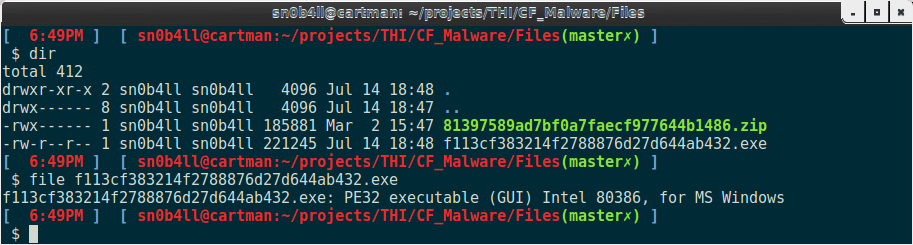
\includegraphics[width=\textwidth]{bilder/statischeAnalyse/fileAuff113.png}
	\caption{Anwendung des File-Kommandos auf die Datei \textit{f113}}
	\label{img:FileAuff113}
\end{figure}

\subsection{Virustotal}
\label{ref:statAnVirustotal}
Im Anschluss kann das Sample \textit{f113} auf \textit{Virustotal} (siehe Sektion \ref{ref:ToolsVirustotal}) hochgeladen werden. Das Ergebnis ist, dass bereits 44 von 56 Virenscannern das Sample erkennen. Als Malware-Familie (nach \textit{NOD32}) wird \textit{Win32/Emotet.AD} angegeben. Ebenso werden alternative Dateinamen wie 
\begin{itemize}
	\item Telekom\_Rechnung\_2015\_02\_de\_04349\_AIEO\_POP\_MAIL\_W5\_5[...]H.exe
	\item dhl\_paket\_de\_003407293054131348371\_02\_2015\_HD\_38300\_J[...]MAIL.exe
\end{itemize} angegeben. Daraus lässt sich schließen, dass die Malware bereits in anderen Spam-Angriffen Anwendung fand. Es werden ebenfalls weiterführende Informationen zum Sample geliefert, welche jedoch im Folgenden über lokale Tools erarbeitet werden. Dies hat den Hintergrund, dass, falls man Opfer eines gezielten Angriffs ist, das Sample nicht umgehend bei Virustotal veröffentlicht werden sollte. Ein Angreifer könnte regelmäßig prüfen, ob das Sample Virustotal bereits bekannt ist. Ist das Sample online, weiß der Angreifer, dass man einen ersten Verdachtsmoment hat und beginnt eventuell damit, seine Spuren zu verwischen.

\subsection{Resource Hacker}
\label{ref:StatAnResourceHacker}
Nun findet das \textit{Resource Hacker} (siehe Abschnitt \ref{ResourceHacker}) Anwendung. Hierzu öffnet man die Anwendung und lädt anschließend über \textit{File} $\rightarrow$ \textit{Open} die Datei \textit{f113}.
\begin{figure}[htbp]
	\centering
	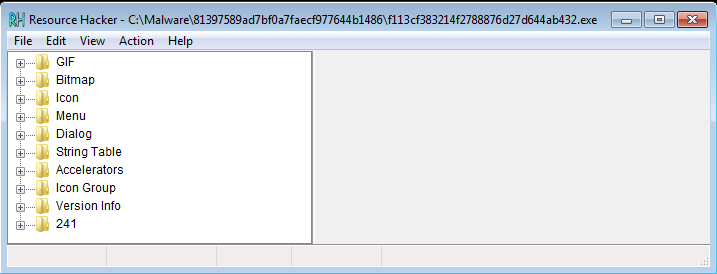
\includegraphics[width=\textwidth]{bilder/statischeAnalyse/ResourceHacker.png}
	\caption{Anwendung des Tools \textit{Resource Hacker} auf die Datei \textit{f113}}
	\label{img:FileAufZip}
\end{figure}
In den jeweiligen Kategorien lassen sich verschiedene Informationen darstellen. Insbesondere drei Informationen fallen bei der Analyse des Files \textit{f113} auf.
\begin{description}
	\item[1. Version Info:]Im Feld \textit{Version Info} wird die Versions-Information des bekannten First-Person-Shooters \textit{Half-Life} von \textit{Valve}\footnote{\url{http://store.steampowered.com/app/70}} verwendet. Der volle Text ist im Anhang unter \ref{ref:versionInfo} zu finden. Diese Maßnahme wird vermutlich verwendet, um die Malware zu tarnen. Durch die kleinste Veränderung von Inhalten wird der Hash der Datei verändert, wodurch primitive Vergleiche das Sample nicht mehr erkennen würden. Zudem können Anti-Viren-Herstellter schlecht den Text als Pattern hinterlegen, da sonst in Zukunft die ausführbare Datei des Spiels \textit{Half-Life} als Malware erkannt werden könnte. Dies wäre ein sogenanntes \textit{False-Positive}, also eine Datei, welche keine Malware ist aber als solche erkannt wird. Im Allgemeinen versuchen Anti-Viren-Hersteller dies zu vermeiden, da sonst die Akzeptanz der Produkte sinkt.
	
	\item[2. Icon:] Im Feld \textit{Icon} kann das in der Abbildung \ref{img:Iconf113} gezeigte Icon gefunden werden. Es zeigt das Logo des \textit{Akrobat Readers}\footnote{\url{https://get.adobe.com/de/reader/otherversions/}}. Es wurde vermutlich gewählt, um den Nutzer den Eindruck zu vermitteln, es würde sich um eine \textit{PDF}-Datei handeln, welche zumeist mit dem \textit{Akrobat Reader} geöffnet werden. Durch die weite Bekanntheit des \textit{Akrobat Readers} erreichen die Malware-Ersteller so eine höhere Quote der Fälle, in welchen die Malware geöffnet wird.
	
\begin{figure}[htbp]
	\centering
	
\includegraphics[scale=1]{bilder/statischeAnalyse/Icon.png}
	\caption{Icon der Datei \textit{f113}}
	\label{img:Iconf113}
\end{figure}

	\item[3. Menü-Bestandteile:] In den Feldern \textit{Bitmap}, \textit{Menu} und \textit{Dialog} können Bestandteile eines Menüs gefunden werden. Die Abbildung \ref{img:Bitmapf113} zeigt das unter \textit{Bitmap} zu findende Bild, welches eine herkömmliche Werkzeugleiste eines Programms zeigt. Unter dem Punkt \textit{Menu} kann zudem ein volles Menü mit asiatischen Schriftzeichen gefunden werden. \textit{Resource Hacker} erlaubt es hier, sich das Menü, wie es im Programm eingebetet wäre, zu inspizieren. Es zeigt sich ein normales Menü, aus dem man, auch ohne die Schriftzeichen zu verstehen, normale Felder wie Öffnen, Speichern oder Schließen ableiten kann (siehe Abbildung \ref{img:Menuf113}). Die Beweggründe, warum das Menü enthalten ist, können unterschiedlich sein. Es könnte direkt vom Programm stammen, sodass man zum Beispiel durch eine bestimmte Eingabe eine Menü öffnen kann. Alternativ kann es auch nur ein weiteres Element der Malware sein, um das Sample schwer von Pattern erfassbar zu machen. Eine andere Alternative wäre, dass die Malware-Ersteller hier Analysten zu falschen Schlussfolgerungen bringen wollen, zum Beispiel, dass die Malware aus dem asiatischen Raum stammt. Daher sollte mit dieser Information sehr behutsam umgegangen werden und die Thesen später bei einem tieferen Wissen nochmals geprüft werden. Zudem ist unter dem Feld \textit{Dialog} ein kleiner Dialog zu finden, welcher in der Abbildung \ref{img:Dialogf113} dargestellt ist.
	
	\begin{figure}[htbp]
		\centering
		
\includegraphics[scale=1]{bilder/statischeAnalyse/Bitmap.png}
		\caption{Enthaltenes Bitmap der Datei \textit{f113}}
		\label{img:Bitmapf113}
	\end{figure}
	\begin{figure}[htbp]
		\centering
		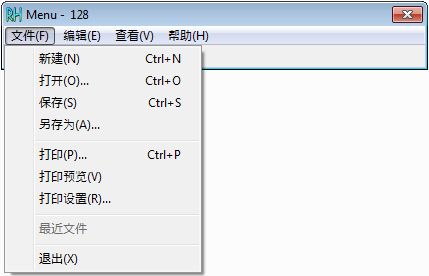
\includegraphics[scale=0.5]{bilder/statischeAnalyse/Menu.png}
		\caption{Enthaltenes Menü der Datei \textit{f113}}
		\label{img:Menuf113}
	\end{figure}
	\begin{figure}[htbp]
		\centering
		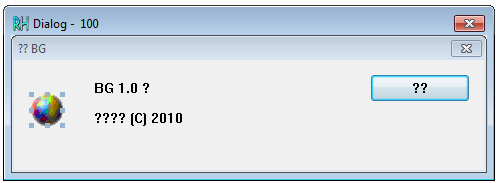
\includegraphics[scale=0.5]{bilder/statischeAnalyse/Dialog.png}
		\caption{Enthaltener Dialog der Datei \textit{f113}}
		\label{img:Dialogf113}
	\end{figure}
\end{description}

\subsection{Dependency Walker}
\label{ref:DependencyWalker}
Als nächstes wird die Datei \textit{f113} mit der Software \textit{Dependency Walker} (siehe Beschreibung \ref{ref:dependencyWalker}) untersucht. Dazu öffnet man den Dependency Walker und öffnet über \textit{File} $\rightarrow$ \textit{Open} die Datei \textit{f113}. Daraufhin zeigt \textit{Dependency Walker} alle verwendeten \textit{DLLs}, sowie deren genutzte Funktionen an. Das Ergebnis ist im Anhang in der Abbildung \ref{img:depWalkerf113} zu sehen. Aus den aufgerufenen Funktionen der \textit{Kernel32.dll} kann man auf die Funktionsweise der Malware schließen. Die interessanten Funktionen sind im Folgenden aufgeführt:
\begin{description}
\item[CompareStringA:] Es wird ein String-Vergleich angestellt. Dies könnte in vielen Szenarien zum Einsatz kommen. Möglichkeiten wären hier ein Vergleich um zu erkennen, ob die Malware in einer VM ausgeführt wird oder ein einfacher Vergleich, in welchem Ordner sich die aktuell ausgeführte Datei befindet.

\item[CreateFileW:] Es wird eine Datei auf das Dateisystem geschrieben. Dies könnte zum Beispiel eine Datei sein, welche beim Systemstart ausgeführt wird.

\item[FindNextFileA:] Es wird nach einer Datei gesucht. Dies kann wiederum der Erkennung einer VM dienen, falls zum Beispiel nach einer bestimmten \textit{DLL} gesucht wird, welche nur von \textit{VMWare} (oder \textit{VirualBox}) verwendet wird.

\item[GetModuleFileNameW:] Es wird entweder der Pfad zu einem Modul oder, falls kein Parameter übergeben wurde, die Pfad zur ausgeführten Anwendung zurückgegeben. Dies könnte zusammen mit \textit{CompareStringA} dazu genutzt werden, die aktuelle Position der Datei \textit{f113} abzufragen und ausgehend davon verschiedene Aktionen auszuführen.

\item[GetModuleHandleW:] Über diese Funktion kann auf eine bereits geladene \textit{DLL} zugegriffen werden. Gelingt es der Malware eine \textit{DLL} in den Kontext zu laden, könnte diese damit benutzt werden.

\item[GetStartupInfoW:] Es wird der \textit{StartupInfo}-Vektor abgefragt. Dieser umfasst unter anderem den Rechnernamen, den Titel der Anwendung sowie andere Elemente des Environments.\footnote{\url{https://msdn.microsoft.com/en-us/library/windows/desktop/ms686331(v=vs.85).aspx}}

\item[HeapSize und VirtualAlloc:] \textit{HeapSize} gibt die aktuelle Größe des \textit{Heaps} an. \textit{VirtualAlloc} reserviert Speicherbereiche. Das Besondere an \textit{VirtualAlloc} ist, dass für die reservierten Speicherbereiche \textit{DEP} deaktiviert werden kann.\footnote{\url{http://0xdabbad00.com/2012/12/07/dep-data-execution-prevention-explanation/}} Dies könnte ein Hinweis dafür sein, dass die Malware versucht (eventuell dynamisch nachgeladenen) \textit{Shellcode} auszuführen. Die \textit{HeapSize} kann dazu eine wichtige Information sein (wird jedoch nicht unbedingt benötigt).
\end{description}

Ob durch die Malware alle festgestellten Funktionen ausgeführt werden, lässt sich in der statischen Analyse nur sehr schwer feststellen. Zudem kann der Ersteller der Malware zu jeder Zeit nicht wirklich benötigte Funktionen einschleusen, um die Analyse zu erschweren.
	
\subsection{PEView}
\label{ref:statAnPEView}
Als nächstes wird das Tool \textit{PEView} (siehe Beschreibung \ref{ref:PEView}) angewendet. Dazu wird \textit{PEView} gestartet und die Datei \textit{f113} ausgewählt. Daraufhin werden im \textit{PEView}-Fenster die verschiedenen Sektionen der ausführbaren Datei anzeigt, wie zu sehen in Abbildung \ref{img:PEViewf113}. Auffällig waren dabei:
\begin{description}
\item[SECTION .data:] Enthält den Text "Rocal AppWizard-Generated Application". Dieser Text wurde bereits in vielen anderen Malware-Samples gefunden\footnote{\url{https://www.google.de/search?q=Rocal+AppWizard}} und wird auch später noch in der Registry auftauchen (siehe Abschnitt \ref{ref:DynAnRegShot}).

\item[SECTION .rsrc:] Enthält den Text "PADDINGXPADDINGXPADDINGX" vielfach. Es lassen sich 2 Funktionen ableiten. Entweder wurde das Padding genutzt, um die ausführbare Datei auf eine korrekte (vom PE/COFF-Format geforderte) Länge zu strecken oder als Padding bei einem möglichen Exploit (siehe \textit{VirtualAlloc} in Sektion \ref{ref:DependencyWalker}).
\end{description}

\begin{figure}[htbp]
	\centering
	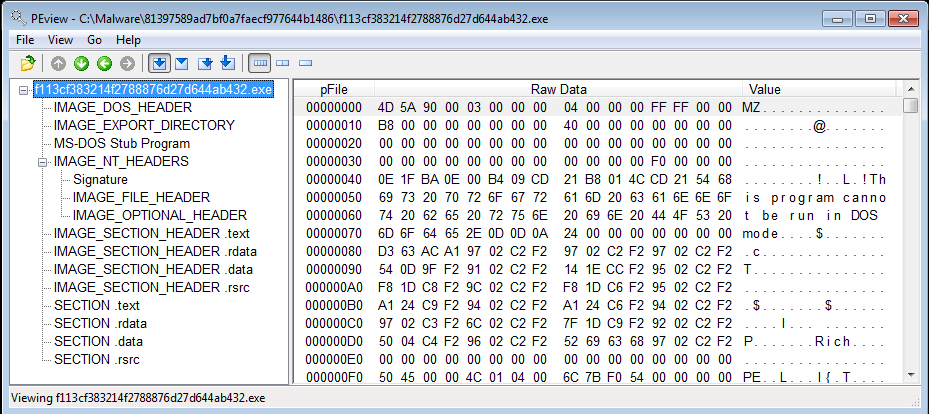
\includegraphics[scale=0.5]{bilder/statischeAnalyse/PEView.png}
	\caption{Aufruf der Datei \textit{f113} mit PEView}
	\label{img:PEViewf113}
\end{figure}
	
Leider liefert \textit{PEView} hier keine weiteren, neuen Informationen zur Datei \textit{f113}.

\subsection{IDA Pro Free}
Als letzten Schritt der statischen Analyse wird die Datei \textit{f113} mit dem Disassembler \textit{IDA PRO Free} (siehe Beschreibung \ref{ref:ToolIDA} untersucht. Dazu öffnen wir die Datei mit dem Programm. Wirft man einen Blick auf die enthaltenen Funktionen, so erkennt man viele, welche für graphische Oberflächen nützlich sind. Beispiele sind im Anhang in der Abbildung \ref{img:IDAFuncf113} aufgezeigt. Auffällig ist, dass viele der Funktionen anscheinend nicht aufgerufen werden oder nur im \textit{.rdata}-Segment verankert sind. Das diese Funktionen im Disassembler nicht genutzt werden, heißt jedoch nicht, dass das Programm in der Ausführung diese nicht dynamisch zur Laufzeit nutzt.
	
Die Analyse, beginnend mit der \textit{start}-Funktion, welche durch den Eintrittspunkt in das Programm ermittelt wird, ergibt folgendes:
\begin{description}
	\item[Funktion \textit{start}:] Es wird zu Anfang die Unterfunktion \textit{sub\_402718} aufgerufen, welche im weiteren Verlauf genauer analysiert wird. Nach dem Aufruf würde das Programm in Unterfunktion \textit{loc\_402C05} springen, in welcher ein neuer Thread erstellt wird. Danach endet das Programm.
	
	\item[Funktion \textit{sub\_402718}:] Die Funktion \textit{sub\_402718} ist wesentlich komplexer (siehe Abbildung \ref{img:IDASub402718f113}). Aktionen in der Klasse sind:
	\begin{enumerate}
		\item Es wird der Applikationstyp über \textit{set\_app\_type}\footnote{\url{https://msdn.microsoft.com/en-us/library/ff770596.aspx}} gesetzt.
		
		\item Anschließend werden einige Variablen und Vektoren initialisiert. Im Anschluss wird ein Sprung genommen, welcher dem Autor auf den ersten Blick nicht ersichtlich ist

\begin{lstlisting}
call    _initterm
add     esp, 24h
mov     eax, ds:_wcmdln
mov     esi, [eax]
cmp     esi, ebx
jnz     short contWithSub
\end{lstlisting}

	Fällt der Vergleich negativ aus, springt das Programm über eine kurze Unterroutine zurück in die \textit{start}-Funktion. Ist der Vergleich positiv, fährt die Funktion \textit{sub\_402718} fort und wird, wie sich später zeigt, nicht mehr in die start-Funktionen zurückkehren.
	
	\item Im Anschluss fährt das Programm über verschiedene Sub-Funktionen fort, welche vermutlich eine Schleife beinhalteten und weitere Variablen initialisiert (in der Abbildung \ref{img:IDASub402718f113} knapp nach der Hälfte zu sehen).
	
	\item Daraufhin wird die \textit{GetStartupInfoW} geladen und verglichen. Der Vergleich bestimmt jedoch nur, ob \textit{0Ah} oder der Wert an der Adresse\\ \textit{ebp+StartupInfo.wShowWindow} als Parameter für die nächste Funktion genutzt wird. Mit welchem Wert die \textit{StartupInfo} verglichen wird, ist leider nicht ersichtlich.
	
	\item Im weiteren Verlauf wird die Funktion \textit{GetModuleHandleW} aufgerufen, welche den \textit{Handle} auf ein Modul lädt. Welches dies genau ist, ist leider in \textit{IDA} nicht ersichtlich.
	
	\item Im Anschluss wird die (selbst-benannte) Funktion \textit{openWindow} aufgerufen, welche intern die Funktion \textit{AfxWinMain()} aufruft. Dadurch wird sehr wahrscheinlich ein Fenster erstellt. Die Funktion kehrt anschließend in die Funktion \textit{sub\_402718} zurück.
	
	\item Dort wird als letztes die Funktion \textit{exit} aufgerufen, welche das Programm beendet.
	\end{enumerate}
\end{description}

\begin{figure}[htbp]
	\centering
	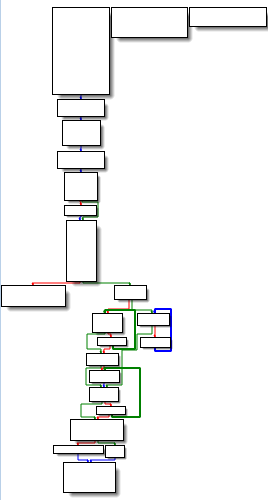
\includegraphics[scale=0.25]{bilder/statischeAnalyse/IDASub402718.png}
	\caption{Funktion sub\_402718 der Datei \textit{f113}, Ansicht in IDA Graphview}
	\label{img:IDASub402718f113}
\end{figure}

Anmerkung: Die statische Disassemblierung gibt eine grobe Einsicht in das Programm, kann aber niemals allen Sprüngen folgen. Es werden von Malware-Entwicklern oft Techniken genutzt, welche die statische Disassemblierung wesentlich erschweren (dynamisches Laden von Programmteilen, Verschlüsselung kritischer Abschnitte oder Ähnliches). Auch hier wurde sehr sicher nicht der volle Funktionsumfang erfasst, da der Thread nur mit wesentlich erhöhtem Aufwand nachverfolgt werden kann.

\subsection{Fazit zur statischen Analyse}
\label{ref:statAnFazit}
Die statische Analyse gab folgende Informationen
\begin{itemize}
\item Die Malware versucht das Opfer glauben zu lassen, sie wäre ein PDF. (siehe \ref{ref:StatAnResourceHacker})
\item Die Malware benutzt die Daten eines Videospiels als Versions-Informationen. (siehe \ref{ref:StatAnResourceHacker})
\item Die Malware beinhaltet Menü-Elemente. (siehe \ref{ref:StatAnResourceHacker})
\item Die Malware stellt Vergleiche an und erstellt eine oder mehrere Dateien. Ebenso führt sie eventuell Shellcode aus. (siehe \ref{ref:DependencyWalker})
\end{itemize}
	\section{Dynamische Analyse}
Die dynamische Analyse gewinnt, im Gegensatz zur statischen Analyse, über die Ausführung der Malware weitere Informationen. So können Verhaltensmuster, welche in der statischen Analyse nur grob vorherzusehen sind, beobachtet und weiter analysiert werden. Im Folgenden werden verschiedene Möglichkeiten und Tools zur dynamischen Analyse vorgestellt.

\subsection{Malwr}
Als erster Punkt der statischen Analyse wird die Datei \textit{f113} auf der Seite \textit{Malwr} (siehe Abschnitt \ref{ref:ToolsMalwr}) analysiert.

Dabei weist \textit{Malwr} auf folgende Eigenheiten hin:
\begin{itemize}
\item File has been identified by at least one AntiVirus on VirusTotal as malicious
\item The binary likely contains encrypted or compressed data.
\item Tries to unhook Windows functions monitored by Cuckoo
\item Executed a process and injected code into it, probably while unpacking
\end{itemize}
Demnach enthält die Datei verschlüsselte Daten, versucht aktiv Sandboxen zu vermeiden und lädt "on-the-fly" Code nach. Dies erklärt, warum die Analyse bisher und im weiteren Verlauf nicht vollständig durchlaufen werden kann. Dem vollständigen Report\footnote{\url{https://malwr.com/analysis/MDIwOTgyODFmOTFiNDU1NDk3ZWFiMzc1NzAwYWI2MGU/}} können weitere Daten entnommen werden.
Aus den gleichen Gründen wie bei \textit{Virustotal}, siehe \ref{ref:statAnVirustotal}, wird nun jedoch ein Großteil der Informationen lokal gesammelt.

\subsection{Live-Analyse}
Als Nächstes folgt die lokale Live-Analyse. Dazu sollte zuallererst ein Snapshot der Virtuellen Maschine erstellt werden, damit man die Maschine nach der Ausführung und Analyse wieder auf einen nicht-kompromittierten Zustand zurücksetzen kann. Im Anschluss werden vor der Analyse folgende Programme gestartet:
\begin{itemize}
	\item RegShot
	\item Process Monitor
	\item Wireshark
	\item Process Explorer
\end{itemize}
Nachdem alle Programme gestartet sind und aufzeichnen, kann die Malware (Datei \textit{f113}) ausgeführt werden. Im Folgenden sind die Ergebnisse aufgezeigt.

\subsubsection{Grundlegende Beobachtungen}
Nach der Ausführung des Programms öffnet sich kein Fenster. Dafür wird die Datei \textit{f113} im ursprünglichen Ordner gelöscht. Es kann keine weitere Aktion beobachtet werden.

\subsubsection{RegShot}
\label{ref:DynAnRegShot}
\textit{RegShot} liefert folgendes Log (gekürzt):
\begin{lstlisting}
Keys added:9 
HKU\S-1-5-21-12[..]00\Software\Microsoft\Multimedia\Audio
HKU\S-1-5-21-12[..]00\Software\Microsoft\Multimedia\Audio\Box
HKU\S-1-5-21-12[..]00\Software\Microsoft\Multimedia\Audio\Box\ba8c80406
HKU\S-1-5-21-12[..]00\Software\Microsoft\Multimedia\Audio\Box\ba8c80407
HKU\S-1-5-21-12[..]00\Software\Microsoft\Multimedia\Audio\Box\ba8c80408
HKU\S-1-5-21-12[..]00\Software\Rocal AppWizard-Generated Applications
HKU\S-1-5-21-12[..]00\Software\Rocal AppWizard-Generated Applications\BG
HKU\S-1-5-21-12[..]00\Software\Rocal AppWizard-Generated Applications\BG\Recent File List
HKU\S-1-5-21-12[..]00\Software\Rocal AppWizard-Generated Applications\BG\Settings
 

Values added:3 
HKU\S-1-5-21-12[..]00\Software\Microsoft\Windows\CurrentVersion\Explorer\UserAssist\{CE[..]EA}\Count\P:\Znyjner\81[..]86\s1[..]32.rkr:
	00 00 00 00 01 00 00 00 00 00 00 00 00 00 00 00 00 00 80 BF 
	00 00 80 BF 00 00 80 BF 00 00 80 BF 00 00 80 BF 00 00 80 BF
	00 00 80 BF 00 00 80 BF 00 00 80 BF 00 00 80 BF FF FF FF FF 
	00 88 32 0C E9 BE D0 01	00 00 00 00
HKU\S-1-5-21-12[..]00\Software\Microsoft\Windows\CurrentVersion\Internet Settings\GlobalUserOffline: 0x00000000
HKU\S-1-5-21-12[..]00\Software\Microsoft\Windows\CurrentVersion\Run\msdb2484d4d.exe: ""C:\Users\Dominik\AppData\Roaming\Microsoft\msdb2484d4d.exe""
\end{lstlisting}

Besonders interessant ist dabei der letzte Eintrag, welcher verrät, dass unter \\ \textit{C:\textbackslash Users\textbackslash Dominik\textbackslash AppData\textbackslash Roaming\textbackslash Microsoft\textbackslash msdb2484d4d.exe} ein neues Programm angelegt wurde, welches beim nächsten Start ausgeführt wird. Prüft man den Hash der Datei, entspricht dieser der Datei \textit{f113}, \textit{f113cf383214f2788876d27d644ab432}. Daher wird die Datei im Folgenden \textit{msdb} genannt. Diese wird unter dem oben genannten Pfad gehalten, um das Verhalten der Malware nicht negativ zu beeinflussen. Ebenfalls fallen die Einträge, welche "`Rocal AppWizard-Generated Applications"' enthalten, auf. Dieser String wurde bereits in der statischen Analyse mit Hilfe von \textit{PEView} unter Abschnitt \ref{ref:statAnPEView} gefunden.

\subsubsection{Process Monitor}
Aus dem \textit{Process Monitor}-Log konnten keine weiteren Kenntnisse gewonnen werden. Das Log ist (gefiltern nach der Datei \textit{f113}) unter \textit{f113cf383214f2788876d27d644ab432.CSV} an die Arbeit angehängt. Es konnte jedoch bestätigt werden, dass die Datei \textit{msdb} geschrieben und zum Autostart hinzugefügt wurde (siehe Abbildung \ref{img:ProcMonf113}). Die Datei \textit{msdb} scheint nicht direkt aufgerufen worden zu sein. Zumindest zeigt der Filter keinen Treffer für \textit{msdb}.

\begin{figure}[htbp]
	\centering
	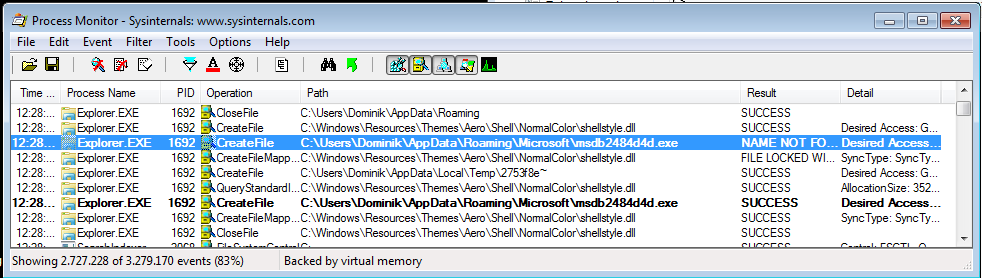
\includegraphics[width=\textwidth]{bilder/dynamischeAnalyse/ProcessMonitor.png}
	\caption{Process Monitor nach Ausführung von \textit{f113} zeigt die Erstellung von \textit{msdb}}
	\label{img:ProcMonf113}
\end{figure}

\subsubsection{Wireshark}
Es konnte kein von der Malware in diesem Stadium ausgelöster Netzwerkverkehr festgestellt werden.

\subsubsection{Process Explorer}
Im \textit{Process Explorer} können Post-Mortem keine Anomalien festgestellt werden. Über das Aufrufen von \textit{Optionen} $\rightarrow$ \textit{Virus Total} $\rightarrow$ \textit{Check Virustotal} können die Hashes aller aktuell laufenden Prozesse gegen die Onlinedatenbank geprüft werden. Dabei wurden alle Prozesse negativ getestet (siehe Abbildung \ref{img:ProcExpf113}). Daraus lässt sich vermuten, dass die Malware zumindest nach der ersten direkten Ausführung nicht mehr läuft. Nachdem die Datei \textit{msdb} jedoch bei einem Neustart des Rechners ausgeführt wird, könnten sich nach einem Neustart neue Funktionen zeigen.

\subsubsection{Autoruns}
Über das Tool \textit{Autoruns} kann die Erkenntnis aus \ref{ref:DynAnRegShot} verifizert werden. Wie unter der Abbildung \ref{img:Autorunsf113} zu sehen ist, wurde ein Autostart-Eintrag für die Datei \textit{msdb} erstellt.

\begin{figure}[htbp]
	\centering
	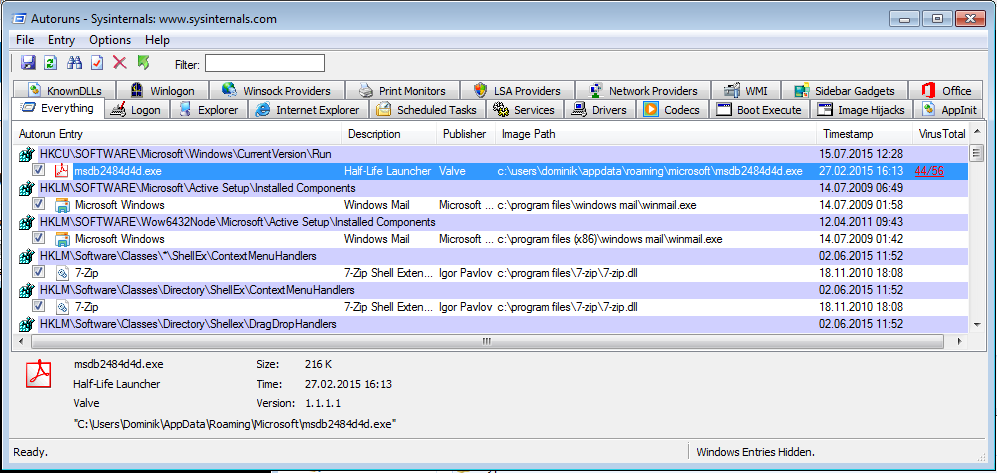
\includegraphics[width=\textwidth]{bilder/dynamischeAnalyse/autoruns.png}
	\caption{\textit{Autoruns} nach Ausführung von \textit{f113}}
	\label{img:Autorunsf113}
\end{figure}

\subsection{Immunity Debugger}
\label{ref:dynAnImmunityDebug}
Nach der Analyse wird die Maschine auf den Zustand vor der Live-Analyse zurückgesetzt. Anschließend wird die Datei \textit{f113} mit dem \textit{Immunity Debugger} (siehe Beschreibung \ref{ref:ToolsImmunityDebugger}) untersucht. Dazu öffnet man das Tool und anschließend die Datei \textit{f113}. Das Fenster ist im Anhang in Abbildung \ref{img:ImmunityDebf113} dargestellt. Anschließend wird über die Tasten \textit{F7} (\textit{Step Into}) und \textit{F8} (\textit{Step Over}) die Ausführung gesteuert. Dabei sind vor allem System-Calls interessant, da diese meist ohne großen Aufwand auf Aktivitäten der Malware schließen lassen.\\[1ex]

Schon zu Beginn lassen sich Parallelen zwischen der Disassemblierung von \textit{IDA} und der Ausführung im Debugger herstellen. Dies ist im Anhang in Abbildung \ref{img:IDAtoImmunityf113} verdeutlicht.\\[1ex]

Später in der Laufzeit kommt man zu der in der statischen Analyse beschriebenen Entscheidung, ob die Unterfunktion \textit{sub\_402718} oder die Start-Funktion weiter ausgeführt werden soll. Die Situation kurz vor dem Vergleich ist im Anhang in der Abbildung \ref{img:IDAtoImmunity2f113} dargestellt. Da \textit{EBX} und \textit{ESI} nicht gleich sind, wird die \textit{Zero}-Flag nicht gesetzt und der Jump (\textit{jnz}) wird normalerweise ausgeführt. Damit würde das Programm in Unterfunktion fortfahren. Das folgende Verhalten gleicht dem bisher beschriebene Verhalten. Um zu testen, was passiert, wenn der Vergleich anders ausgeht, wird der Sprung \textit{JNZ} auf \textit{JE} manipuliert (welcher das Gegenstück zu \textit{JNZ} ist). Abbildung \ref{img:ImmunityDebJZf113} zeigt den Assemblercode nach der Anpassung.

\begin{figure}[htbp]
	\centering
	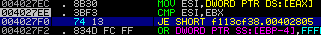
\includegraphics[width=\textwidth]{bilder/dynamischeAnalyse/ImmunityDebug2.png}
	\caption{Veränderung \textit{JNZ} zu \textit{JZ} während der Ausführung von \textit{f113}}
	\label{img:ImmunityDebJZf113}
\end{figure}

Leider führt diese weitere Ausführung auf eine \textit{Access-Violation}. Da Programme gezielt gegen Debugging geschützt werden können und eine solche Methode hier vermutlich zum Einsatz kommt, wurde die weitere Ausführung aufgegeben.

\subsection{Weiter Analyse}
Um das weitere Verhalten der Datei \textit{msdb} zu analysieren, wurden \textit{Process Monitor} und \textit{Wireshark} herangezogen. Zur Analyse der Datei \textit{msdb} bei einem Neustart wird im \textit{Process Monitor} die \textit{Option} $\Rightarrow$ \textit{Enable Boot Logging} aktiviert. Nach einem Neustart kann man nun die während der Bootzeit ausgeführten Aktionen analysieren.\\[1ex]

Wireshark zeigt wiederum keinen auffälligen Netzwerkverkehr. Das Log des \textit{Process Monitor} (welches nach dem Öffnen der Software nach dem Neustart angeboten wird) zeigt zwar, dass die Datei \textit{msdb} geladen wurde, zeigt aber keine weiteren Aktionen. Im \textit{Prozess Explorer} kann die Datei \textit{msdb} ebenfalls nicht als laufendes Programm gefunden werden.

\newpage
\subsection{Fazit zur dynamischen Analyse}
\label{ref:dynAnFazit}
Die dynamische Analyse konnte einige grundlegende Verhalten der Malware in Erfahrung bringen:
\begin{itemize}
	\item Die Ursprungs-Datei \textit{f113} löscht sich nach der Ausführung selbst.
	\item Die Datei \textit{msdb} wird nach der Ausführung von Datei \textit{f113} in den Ordner \\\textit{C:\textbackslash Users\textbackslash Dominik\textbackslash AppData\textbackslash Roaming\textbackslash Microsoft} kopiert.
	\item Für die Datei \textit{msdb} wird ein Autostart-Eintrag unter Software \\
\textit{\textbackslash Microsoft\textbackslash Windows\textbackslash CurrentVersion\textbackslash Run} angelegt
\end{itemize}
Leider konnten, vermutlich aufgrund der Eigenschaft, dass die Malware erkennt, dass sie analysiert wird, nicht alle Funktionalitäten in Erfahrung gebracht werden.
	\section{Fazit}
Durch die statische Analyse ließen sich verschiedene mögliche Funktionen der Malware erschließen (siehe Sektion \ref{ref:statAnFazit}). Daraus lassen sich für Nutzer Sicherheitshinweise ableiten. So sollten diese immer zuerst die Dateiendung überprüfen, und sich nicht von Icons täuschen lassen.\\[1ex]
	
Ebenso konnte über die dynamische Analyse zumindest ein Teil der Funktionalität aufgedeckt werden (siehe Abschnitt \ref{ref:dynAnFazit}). Aus den Erkenntnissen lassen sich \textit{Indicator of Compromise} ableiten. So könnte man zum Beispiel bei dem Verdacht, dass ein Rechner mit der hier analysierten Malware infiziert ist, auf die Datei \textit{msdb} prüfen und die Autorun-Einträge untersuchen.\\[1ex]

Dass keine weiteren Aktivitäten der Malware verzeichnet werden konnten, kann sich auf mehrere Gründe zurückführen lassen. So könnte die Malware nur für eine spezielle Windows-Konfiguration entwickelt worden sein, welche hier nicht geboten wurde. Auch wäre es möglich, dass die Malware sich erst zu einem bestimmten Zeitpunkt aktiviert und bis dahin schläft. Am wahrscheinlichsten ist jedoch, dass die Malware die virtuelle Umgebung erkannt hat und daher nicht seine eigentliche Funktionalität entfaltet. Die Annahme, dass die Malware die VM erkannt hat, wird durch die Analyse von Alexey Shulmin auf \url{securelist.com}\footnote{\url{https://securelist.com/analysis/publications/69560/the-bank\\ing-trojan-emotet-detailed-analysis/}} gestützt.
%---------------Anhang-------------------------------------------
	\newpage
	
%------------------------------------------------------------------------
% Anhänge
\appendix
\section{Appendix}
\subsection{Version Info}
\label{ref:versionInfo}
\begin{lstlisting}
1 VERSIONINFO
FILEVERSION 1,1,1,1
PRODUCTVERSION 1,1,1,1
FILEOS 0x4
FILETYPE 0x1
{
BLOCK "StringFileInfo"
{
	BLOCK "040904b0"
	{
		VALUE "CompanyName", "Valve"
		VALUE "FileDescription", "Half-Life Launcher"
		VALUE "FileVersion", "1, 1, 1, 1"
		VALUE "InternalName", "Half-Life Launcher"
		VALUE "LegalCopyright", "Copyright (c) 1996-2003"
		VALUE "LegalTrademarks", ""
		VALUE "OriginalFilename", "hl.exe"
		VALUE "ProductName", "Half-Life Launcher"
		VALUE "ProductVersion", "1, 1, 1, 1"
	}
}

BLOCK "VarFileInfo"
{
	VALUE "Translation", 0x0409 0x04B0
}
}
\end{lstlisting}

\newpage
\subsection{Abbildungen}

\begin{figure}[htbp]
	\centering
	
\includegraphics[scale=0.5]{bilder/EMail.png}
	\caption{Gefälschte UPS-Mail}
	\label{img:EMail}
\end{figure}

\begin{figure}[htbp]
	\centering
	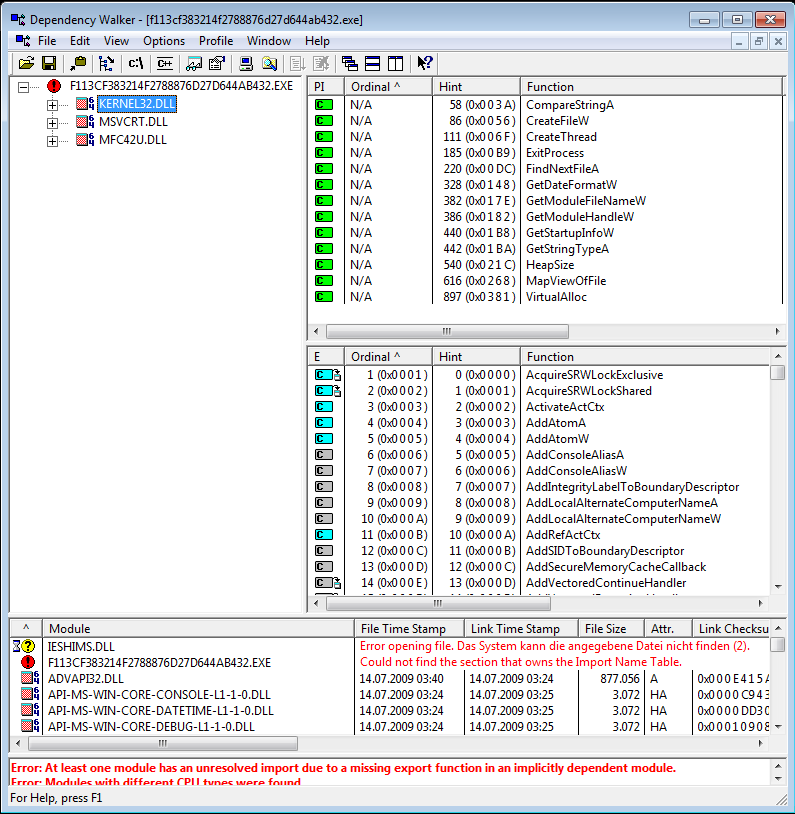
\includegraphics[scale=0.5]{bilder/statischeAnalyse/depWalker.png}
	\caption{Aufruf der Datei \textit{f113} mit dem Dependency Walker}
	\label{img:depWalkerf113}
\end{figure}

\begin{figure}[htbp]
	\centering
	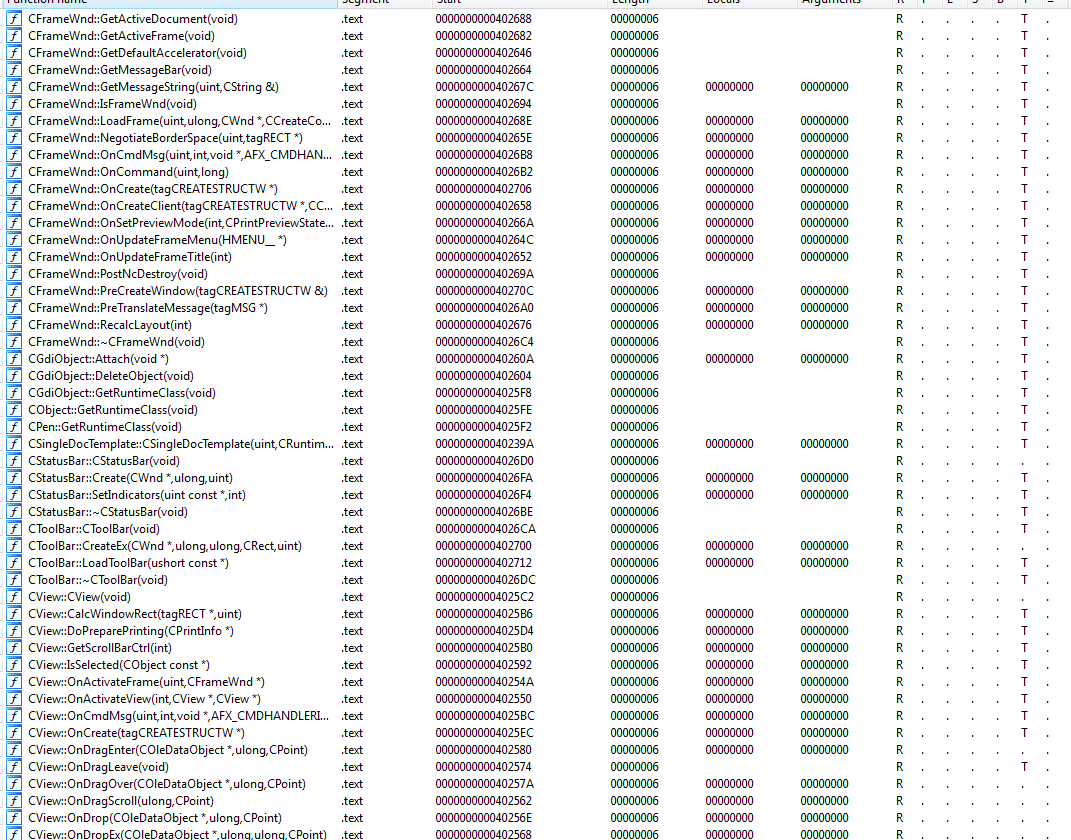
\includegraphics[width=\textwidth]{bilder/statischeAnalyse/IDAFunc.png}
	\caption{Funktionsaufrufe der Datei \textit{f113}, Ansicht in IDA}
	\label{img:IDAFuncf113}
\end{figure}

\begin{figure}[htbp]
	\centering
	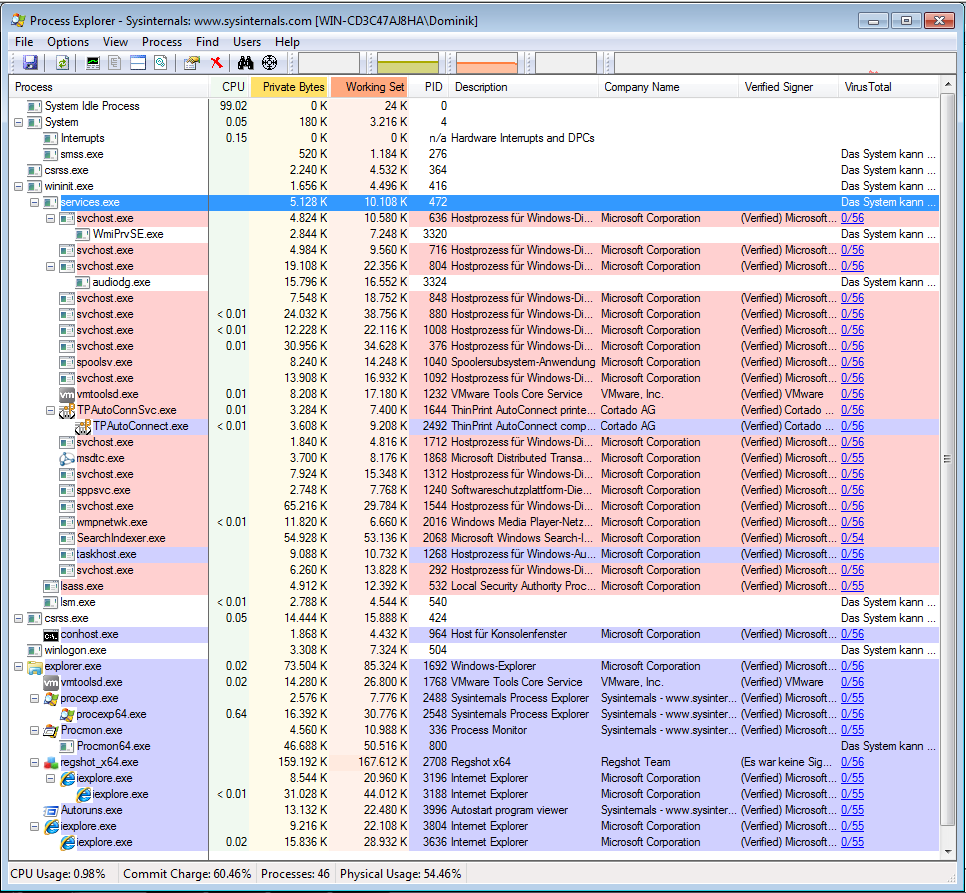
\includegraphics[width=\textwidth]{bilder/dynamischeAnalyse/ProcessExplorer.png}
	\caption{Process Explorer nach Ausführung von \textit{f113} mit Abgleich der Prozesse mit Virustotal}
	\label{img:ProcExpf113}
\end{figure}

\begin{figure}[htbp]
	\centering
	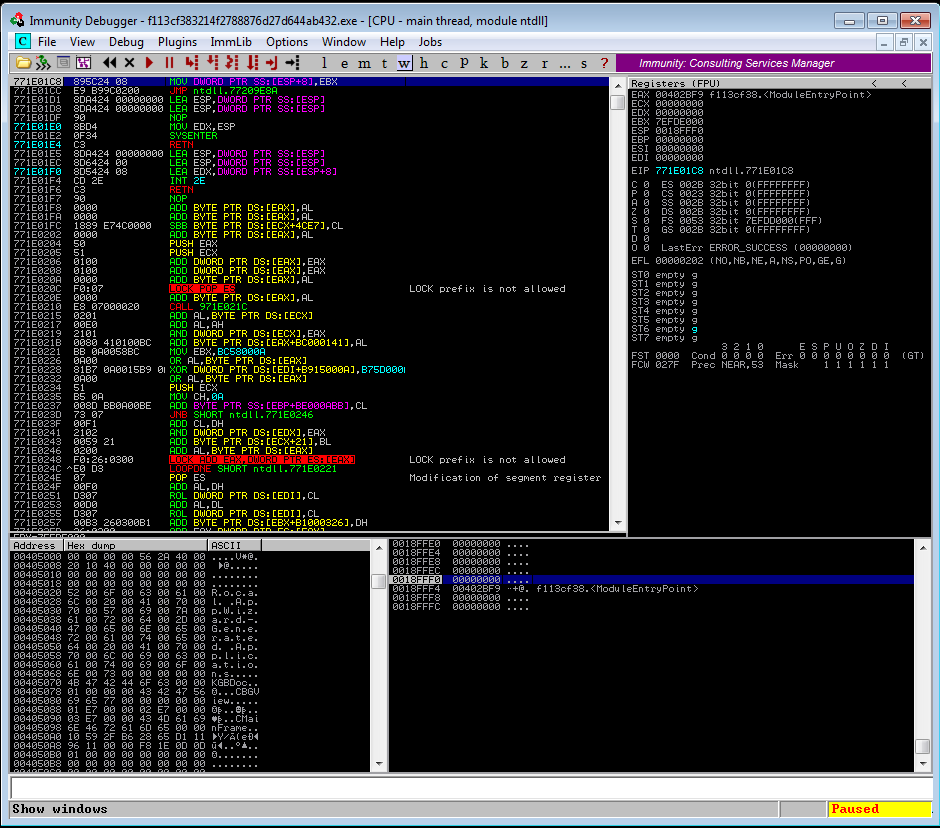
\includegraphics[width=\textwidth]{bilder/dynamischeAnalyse/ImmunityDebug.png}
	\caption{Hauptfenster des \textit{Immunity Debuggers} nach Ausführung von \textit{f113}}
	\label{img:ImmunityDebf113}
\end{figure}

\begin{figure}[htbp]
	\centering
	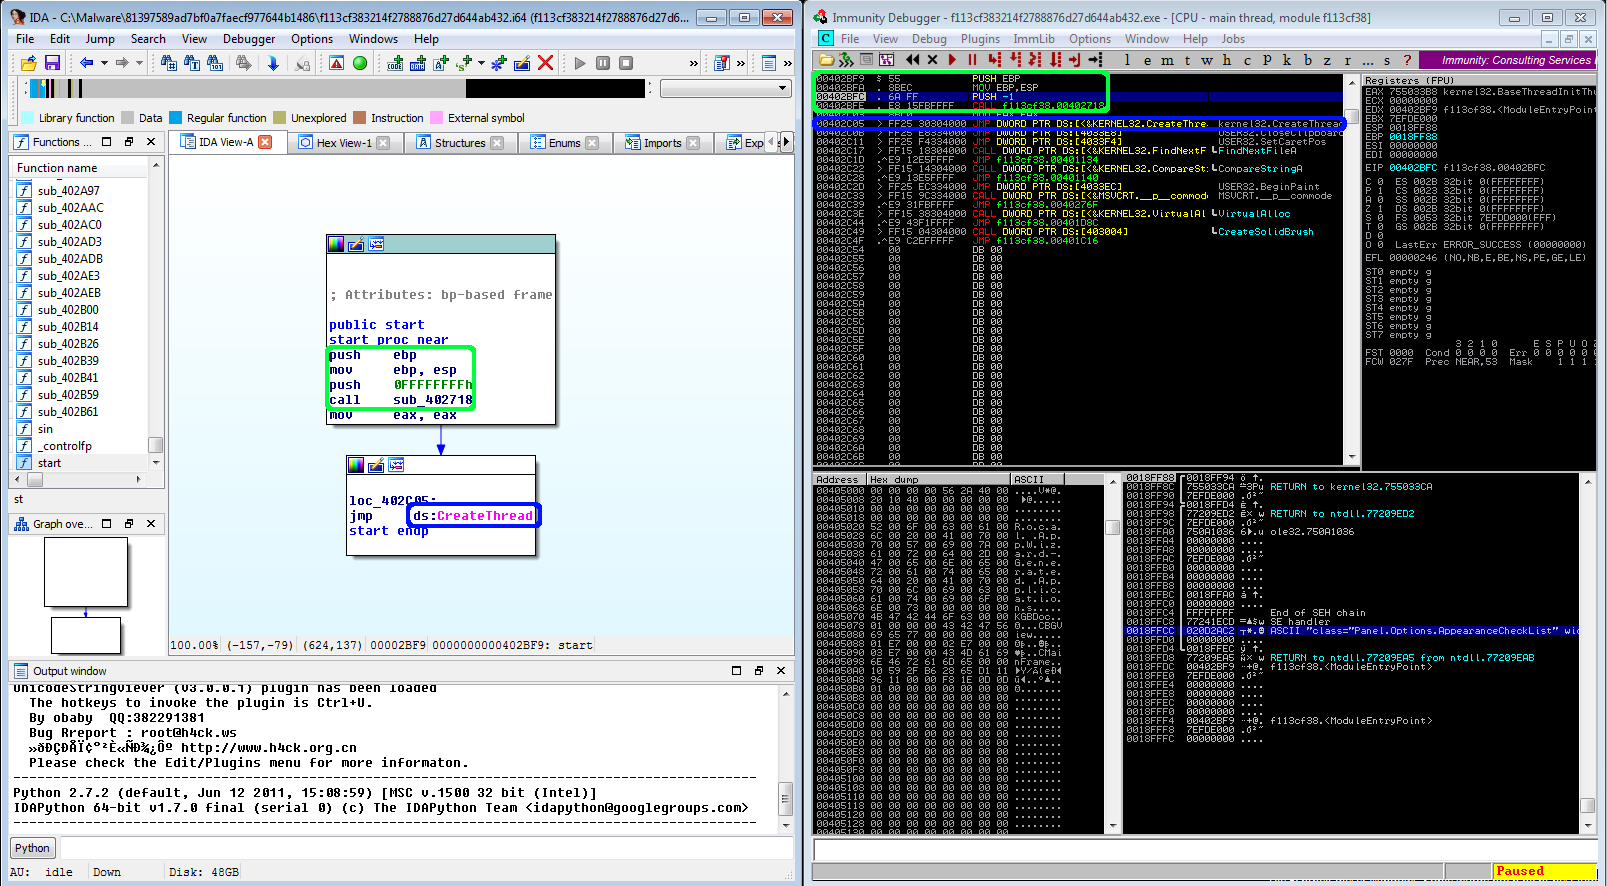
\includegraphics[angle=90, scale=.35]{bilder/dynamischeAnalyse/IDAtoImmunity.png}
	\caption{Zusammenhang von \textit{IDA} und \textit{Immunity Debuggers} bei \textit{f113}}
	\label{img:IDAtoImmunityf113}
\end{figure}

\begin{figure}[htbp]
	\centering
	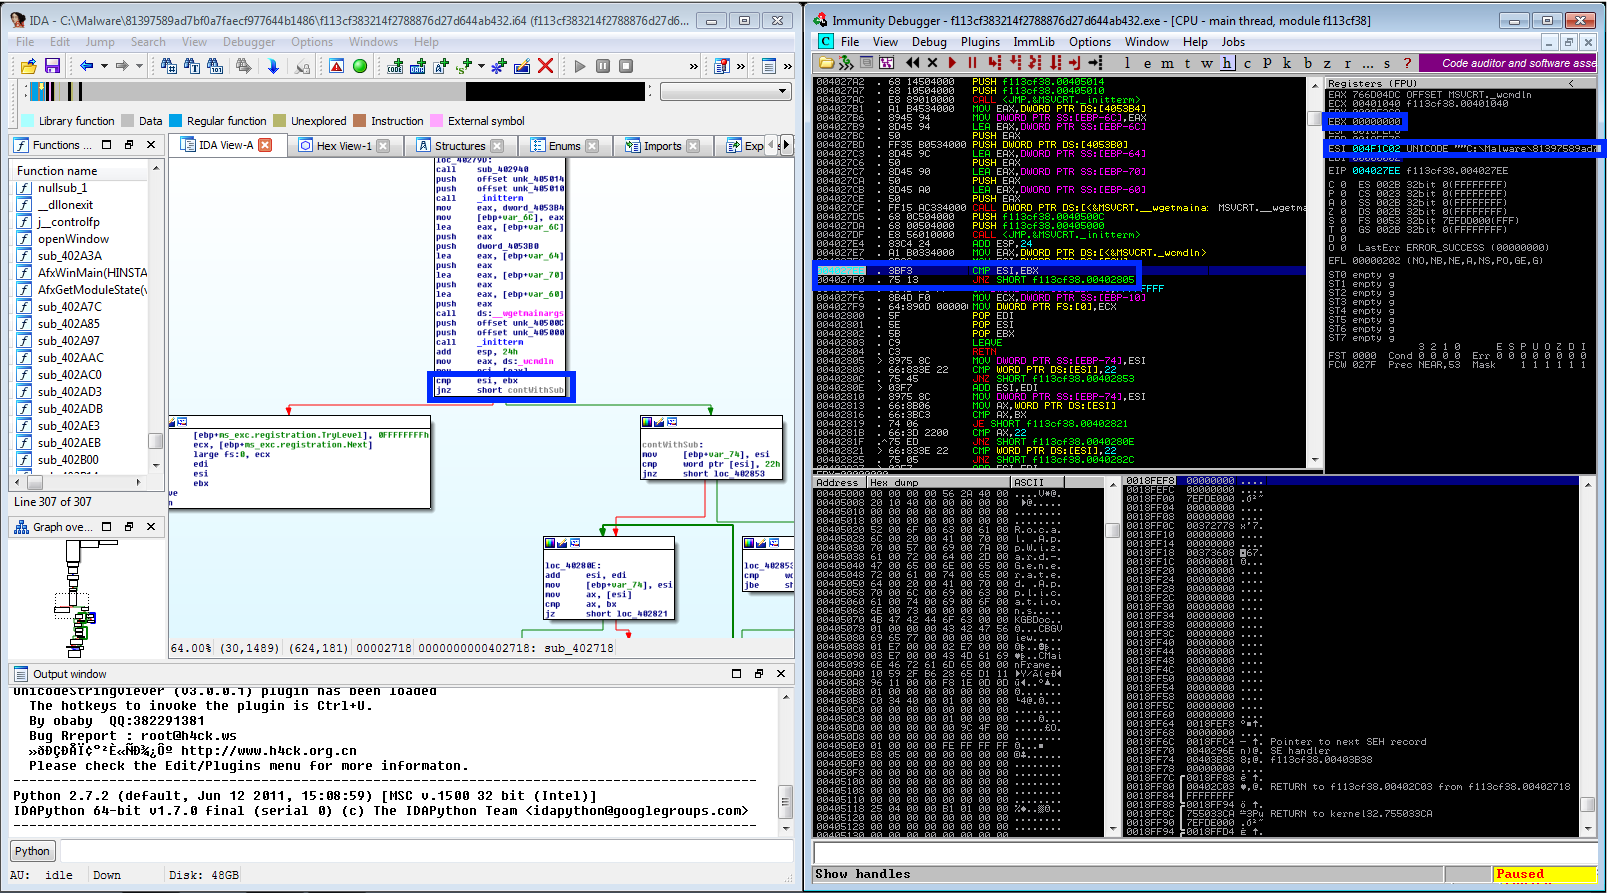
\includegraphics[angle=90, scale=.35]{bilder/dynamischeAnalyse/IDAtoImmunity2.png}
	\caption{Zusammenhang von \textit{IDA} und \textit{Immunity Debuggers} bei \textit{f113}}
	\label{img:IDAtoImmunity2f113}
\end{figure} % Anhang
	\newpage
%	\printbibliography % Literaturliste
\end{document}
%-----------------------------------------------------------------
%---------------Dokumentenende------------------------------------
%-----------------------------------------------------------------
